\documentclass{article}

% para usar codificación utf8
\usepackage[utf8]{inputenc}
% define los márgenes del documento
\usepackage{geometry}
  \geometry{
    a4paper,
    left = 3cm,
    right = 3cm,
    top = 2.5cm,
    bottom = 2.5cm
  }
% se usan para darle color los títulos y subtítulos
\usepackage{titlesec}
\usepackage{color}
% permite añadir imágenes al documento
\usepackage{graphicx}
% usado para operaciones matemáticas
\usepackage{amsmath}
% traduce textos como "figure" al español
\usepackage[spanish]{babel}

% títulos de color azul y subtítulos de color rojo
\titleformat*{\section}{\normalfont\Large\bfseries\color{blue}}
\titleformat*{\subsection}{\normalfont\large\bfseries\color{red}}
% párrafos sin sangría
\setlength\parindent{0pt}

% comandos nuevos para comillas simples y dobles
\newcommand{\simple}[1]{`#1'}
\newcommand{\doble}[1]{``#1''}

\title{Resumen Python 3}
\author{Víctor Mardones Bravo}
\date{Febrero de 2021}

\begin{document}

  % la primera hoja no tiene números de página
  \pagenumbering{gobble}

  % brujería para centrar el título y logo
  \null
  \nointerlineskip
  \vfill
  \let\snewpage \newpage
  \let\newpage \relax
  % se centra el logo svg exportado con Inkscape
  {\centering\def\svgwidth{\columnwidth}
  \input{logo python\\python-logo-inkscape.pdf_tex}}
  \maketitle
  \let \newpage \snewpage
  \vfill 
  \break

  \newpage

  % el resto del documento tiene números de página
  \pagenumbering{arabic}

  \section{Introducción a Python}

    \subsection{¿Qué es Python?}

    Python es un lenguaje de programación de alto nivel, con aplicaciones en numerosas áreas, incluyendo programación web, scripting, computación científica e inteligencia artificial.

    Es muy popular y usado por organizaciones como Google, la NASA, la CIA y Disney.

    No hay limitaciones en lo que se puede construir usando Python. Esto incluye aplicaciones autónomas, aplicaciones web, juegos, ciencia de datos, modelos de machine learning y mucho más.

    Dato curioso: Según el creador Guido van Rossum, el nombre de Python viene de la serie de comedia británica \doble{El Circo Volador de Monty Python}.

    \subsection{El Zen de Python}

      El Zen de Python es una colección de 19 \doble{principios} para escribir programas de computadores que influenciaron el diseño y representan la filosofía de este lenguaje de programación.

      \begin{figure}[ht!]
        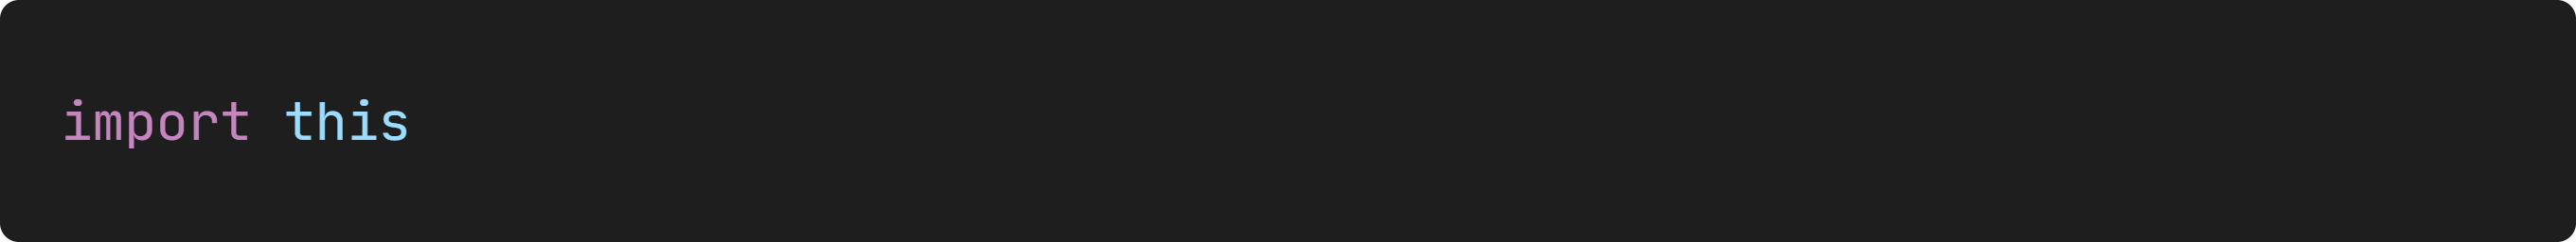
\includegraphics[width=\linewidth]{imagenes\\cap1\\import this.png}
        \caption{El Zen de Python se muestra en pantalla la primera vez que se ejecute esta línea.}
      \end{figure}

      \begin{figure}[ht!]
        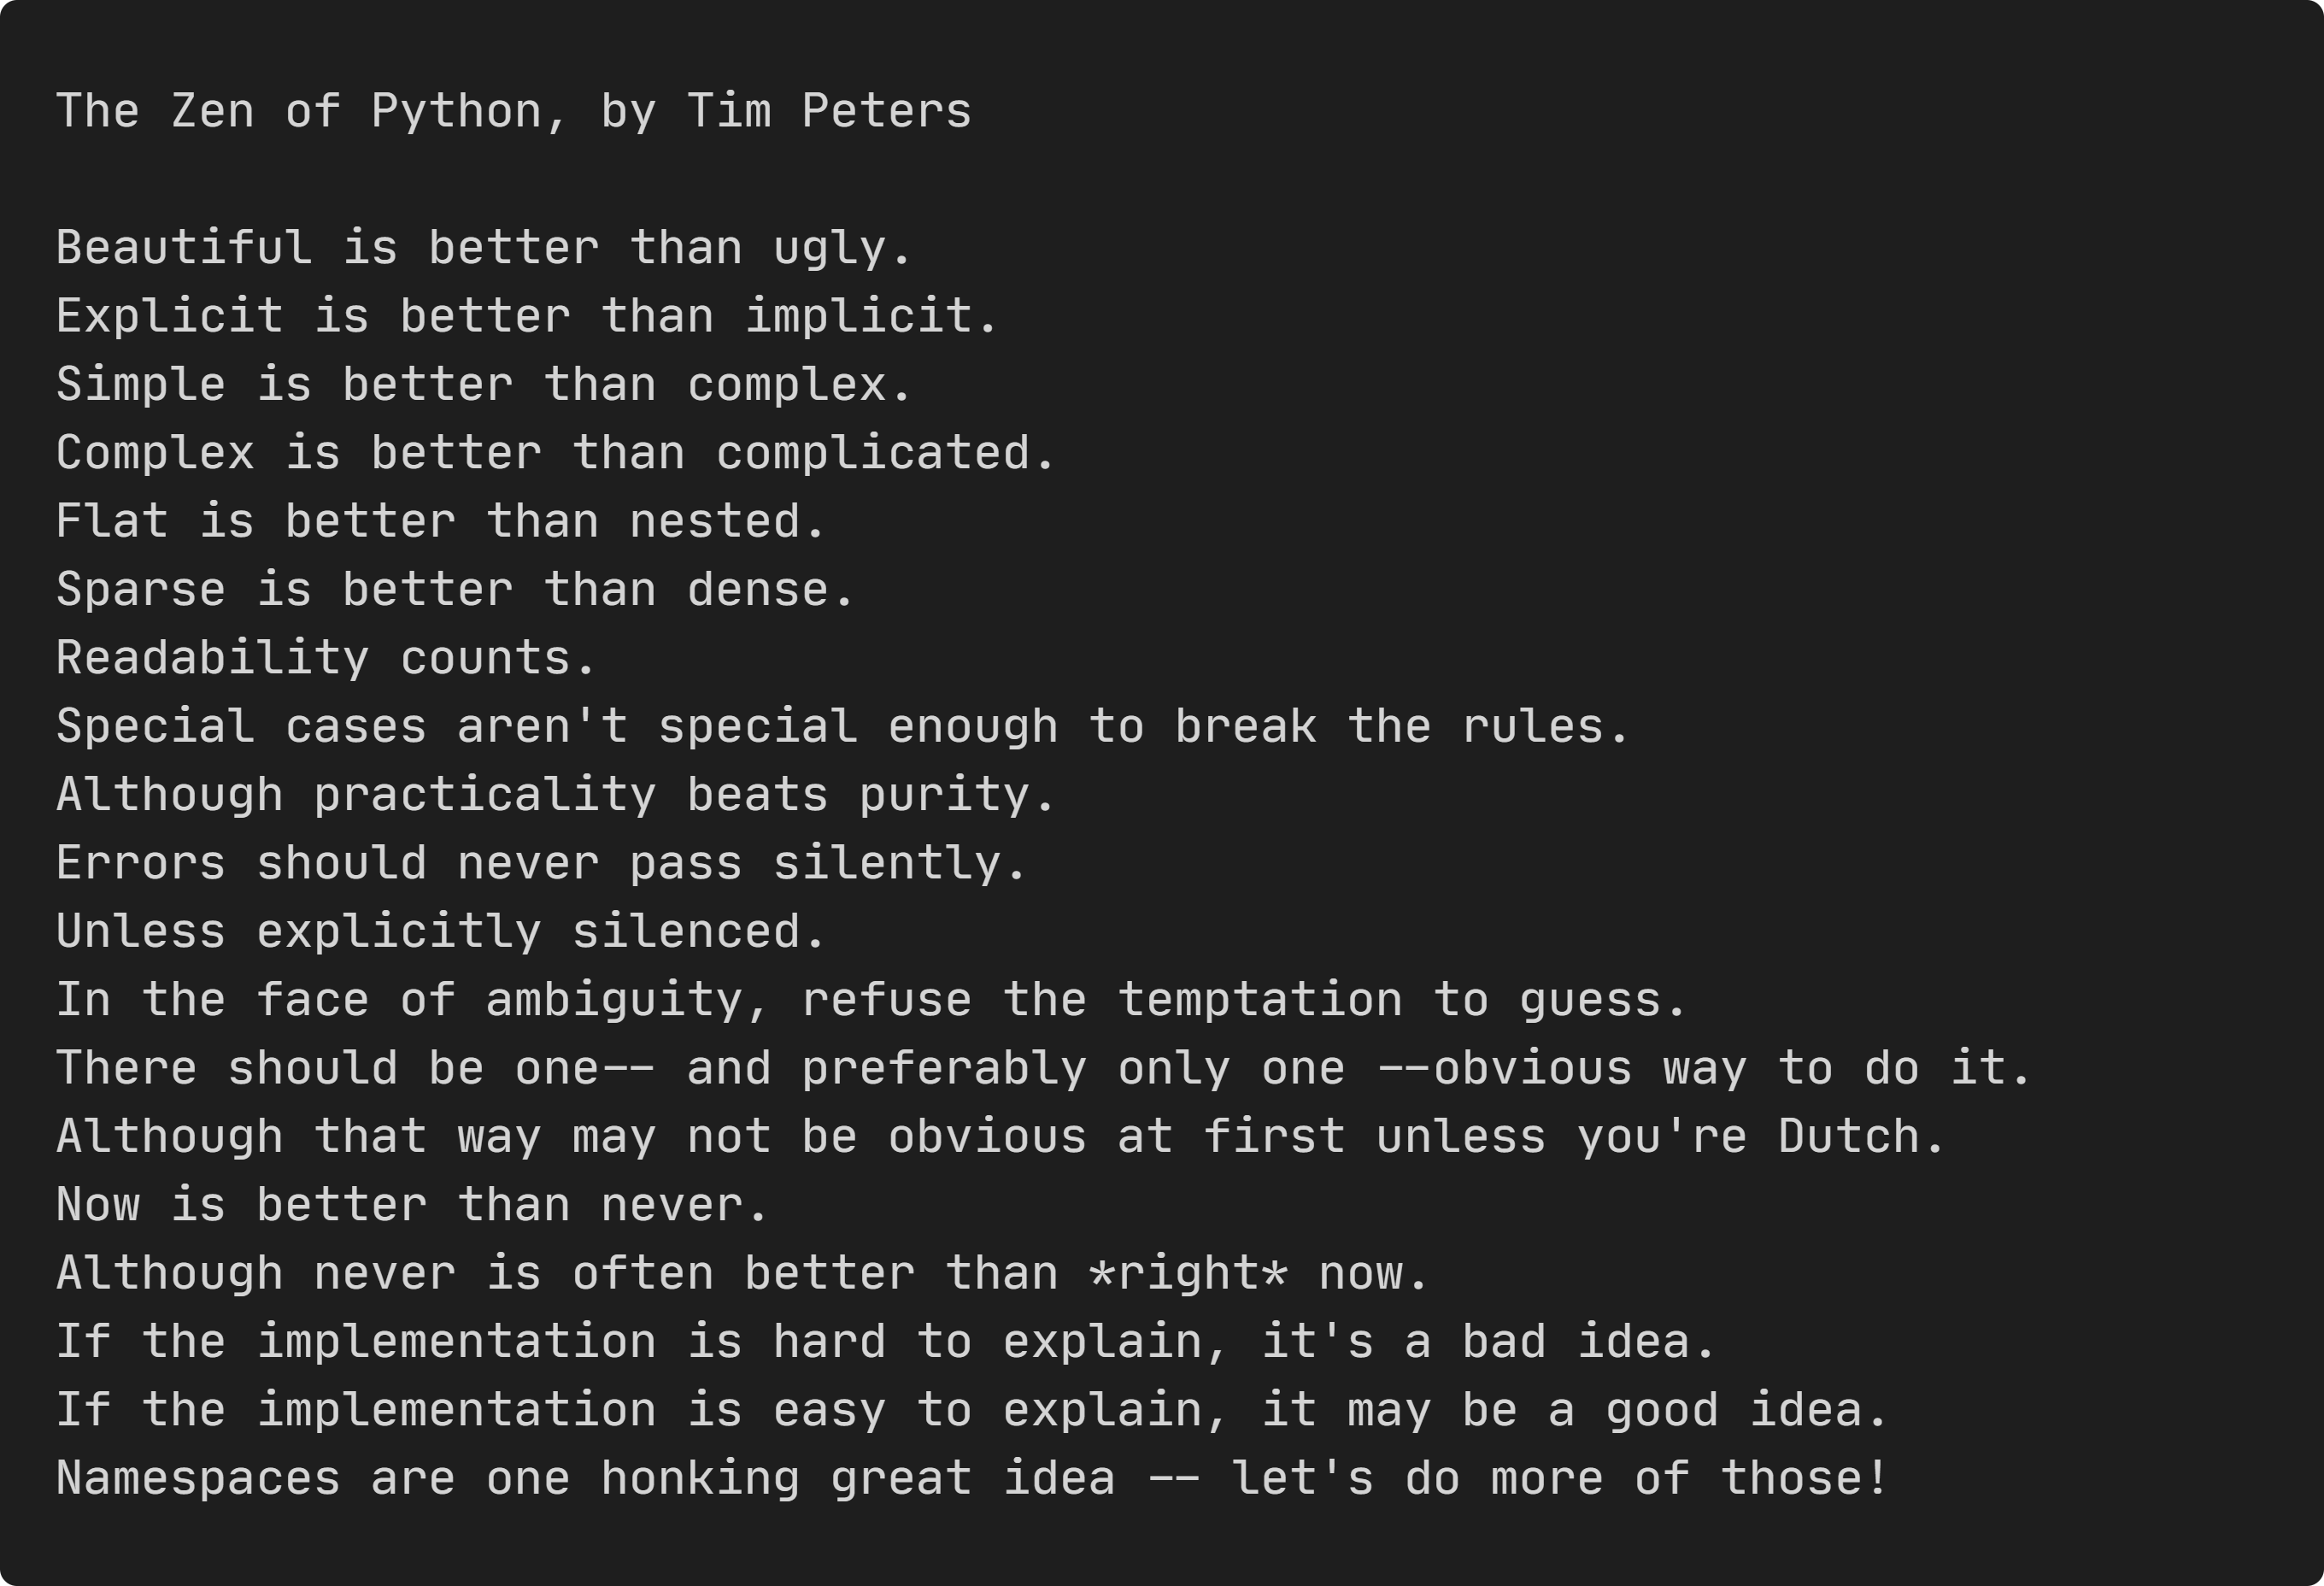
\includegraphics[width=\linewidth]{imagenes\\cap1\\zen.png}
        \caption{El Zen de Python, escrito por Tim Peters.}
      \end{figure}


    \subsection{Hola mundo}

      Para mostrar el texto \doble{Hola mundo} en pantalla se puede usar la función print().

      \begin{figure}[ht!]
        
\includegraphics[width=\linewidth]{imagenes\\cap1\\hola mundo 1.png}
        \caption{Hola mundo, el clásico primer programa en cualquier lenguaje de programación.}
      \end{figure}

      \begin{figure}[ht!]
        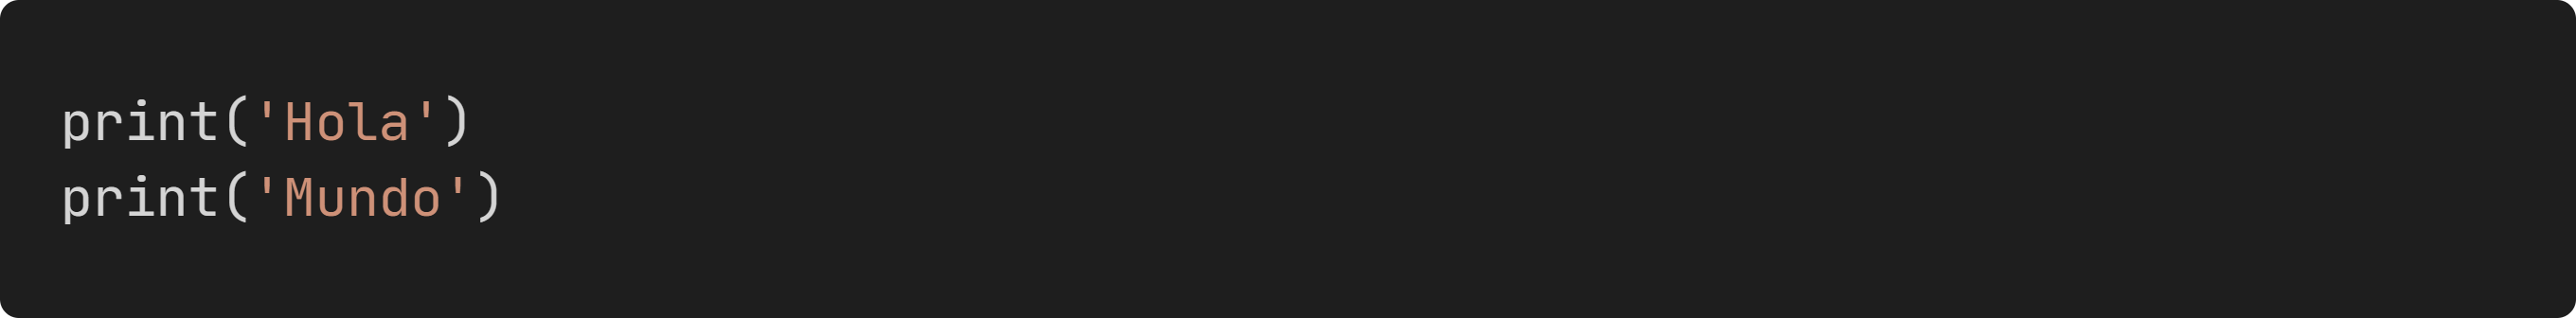
\includegraphics[width=\linewidth]{imagenes\\cap1\\hola mundo 2.png}
        \caption{Cada declaración de impresión print() genera texto en una nueva línea.}
      \end{figure}

  \newpage
  \section{Conceptos básicos}

    \subsection{Comentarios}

      Los comentarios son anotaciones en el código utilizadas para hacerlo más fácil de entender. No afectan la ejecución del código.

      En Python, los comentarios comienzan con el símbolo \#. Todo el texto luego de este \# (dentro de la misma línea) es ignorado.

      \begin{figure}[ht!]
        
\includegraphics[width=\linewidth]{imagenes\\cap2\\comentario.png}
        \caption{Ejemplo de un comentario en Python.}
      \end{figure}

      Python no soporta comentarios multilínea, al contrario de otros lenguajes de programación.

      A lo largo de este resumen, se usarán comentarios para mostrar la salida de algunas funciones, cuando sea posible.

    \subsection{Operaciones aritméticas}
      Python tiene la capacidad de realizar cálculos. Los operadores +, -, * y / representan suma, resta, multiplicación y división, respectivamente.

      \begin{figure}[ht!]
        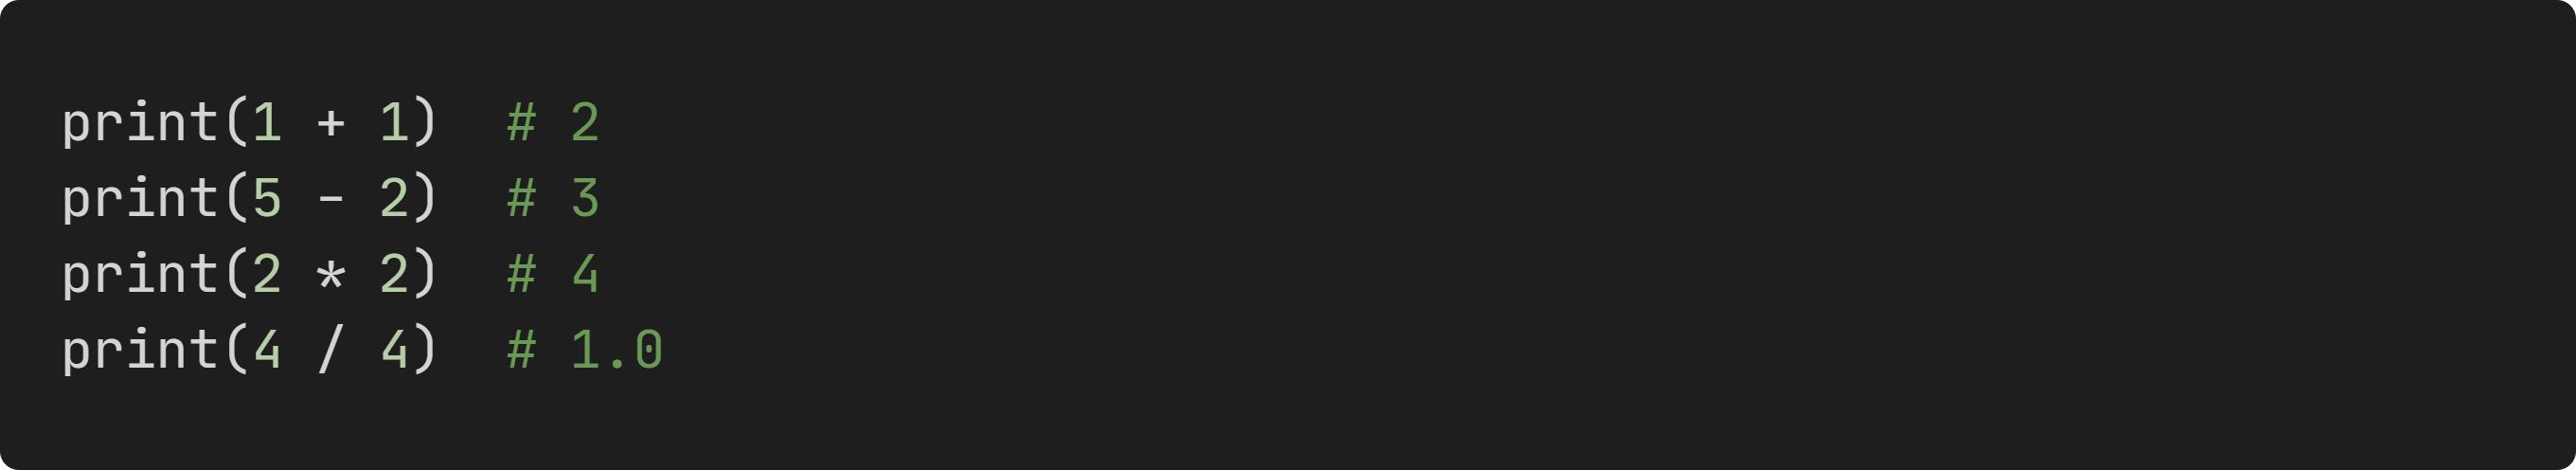
\includegraphics[width=\linewidth]{imagenes\\cap2\\aritmetica 1.png}
        \caption{Adición, sustracción, multiplicación y división en Python.}
      \end{figure}

      Los espacios entre los signos y los números son opcionales, pero hacen que el código sea más fácil de leer.

    \subsection{La regla PEMDAS}
      Las operaciones en Python siguen el orden dado por la regla PEMDAS:

      \begin{enumerate}
        \item Paréntesis
        \item Exponentes
        \item Multiplicación y división
        \item Adición y Sustracción
      \end{enumerate}

      % TODO: aritmetica 2 con ejemplos de operaciones combinadas

    \subsection{Paréntesis}
      Se pueden usar paréntesis () para agrupar operaciones y hacer que estas se realicen primero, siguiendo la regla PEMDAS.

      \begin{figure}[ht!]
        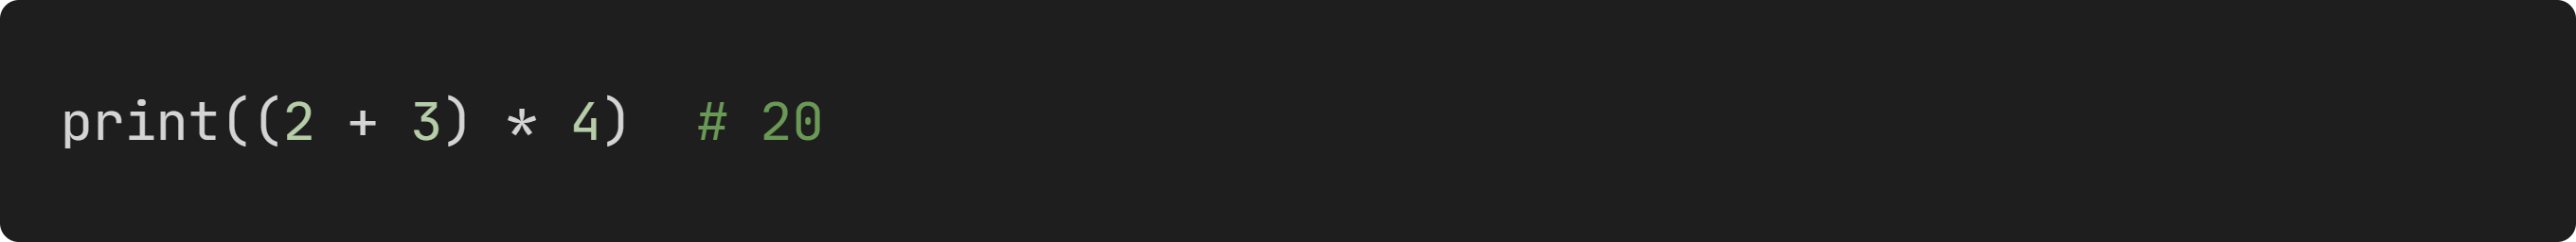
\includegraphics[width=\linewidth]{imagenes\\cap2\\aritmetica 3.png}
        \caption{Uso de paréntesis para cambiar el orden de las operaciones.}
      \end{figure}

    \subsection{Floats}
      Para representar números que no son enteros, se usa el tipo de dato float o punto flotante. Se pueden crear directamente ingresando un número con un punto decimal, o como resultado de una división.

      \begin{figure}[ht!]
        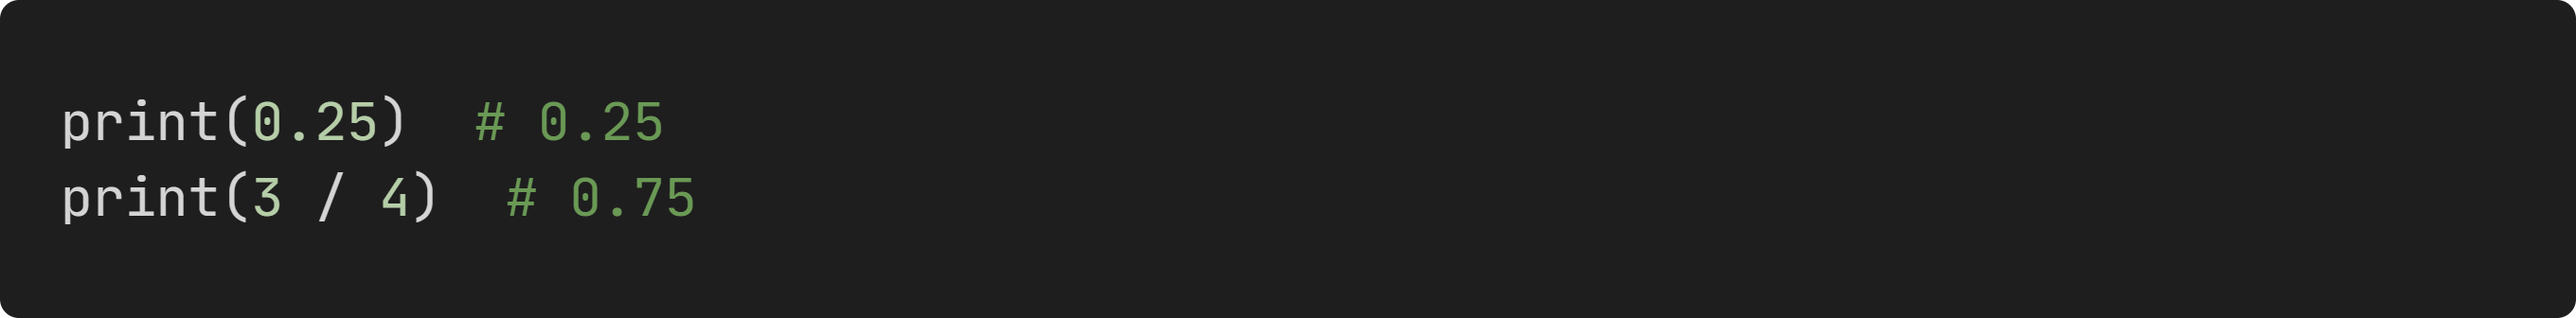
\includegraphics[width=\linewidth]{imagenes\\cap2\\float 1.png}
        \caption{Los floats representan números racionales.}
      \end{figure}

      Se debe tener en cuenta que los computadores no pueden almacenar perfectamente el valor de los floats, lo cual a menudo conduce a errores.

      \begin{figure}[ht!]
        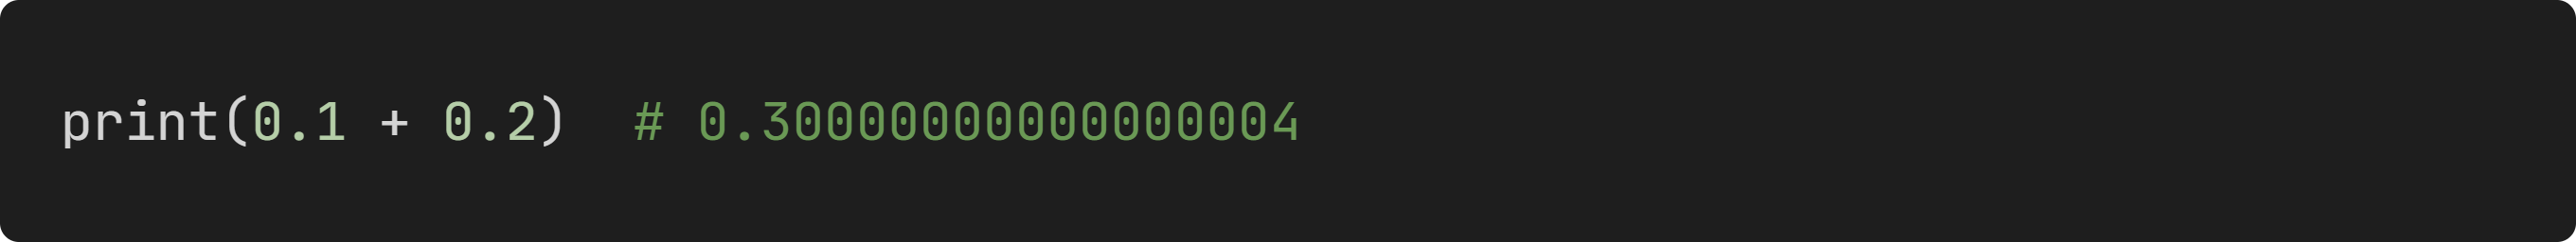
\includegraphics[width=\linewidth]{imagenes\\cap2\\error float.png}
        \caption{Un error clásico de la aritmética de punto flotante.}
      \end{figure}

      Al trabajar con floats, no es necesario escribir un 0 a la izquierda del punto decimal.

      \begin{figure}[ht!]
        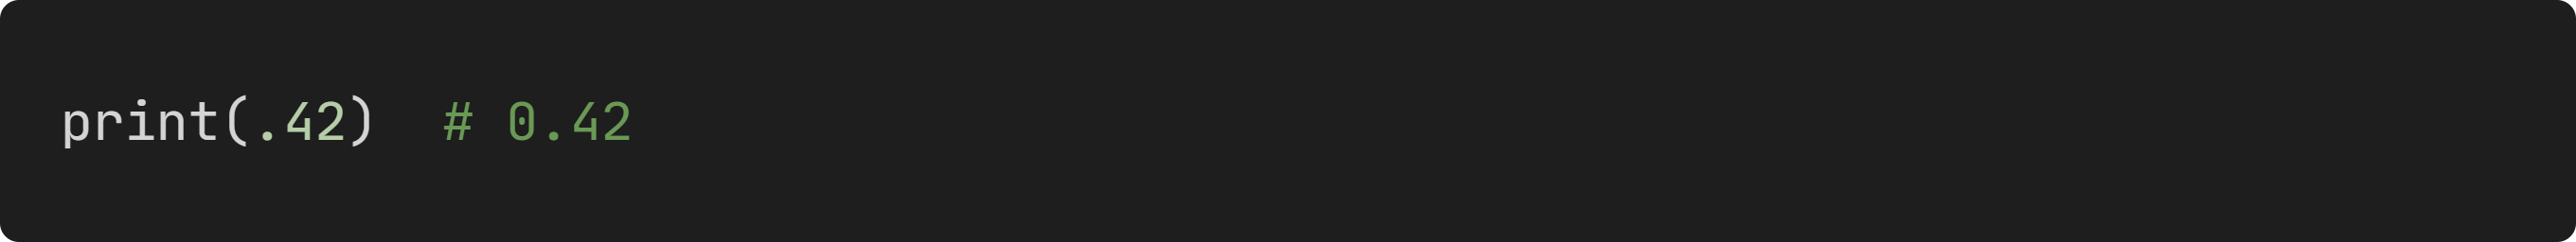
\includegraphics[width=\linewidth]{imagenes\\cap2\\float 2.png}
        \caption{Esta notación se asemeja a decir \doble{punto cinco} en vez de \doble{cero punto cinco}.}
      \end{figure}

      El resultado de cualquier operación entre floats o entre un float y un entero siempre dará como resultado un float. La división entre enteros también da como resultado un float.

      %TODO: float 3 mostrando resultados de operaciones entro floats y enteros

      \subsection{Exponenciación}

      Otra operación soportada es la exponenciación, que es la elevación de un número a la potencia de otro. Esto se realiza usando el operador **.

      \begin{figure}[ht!]
        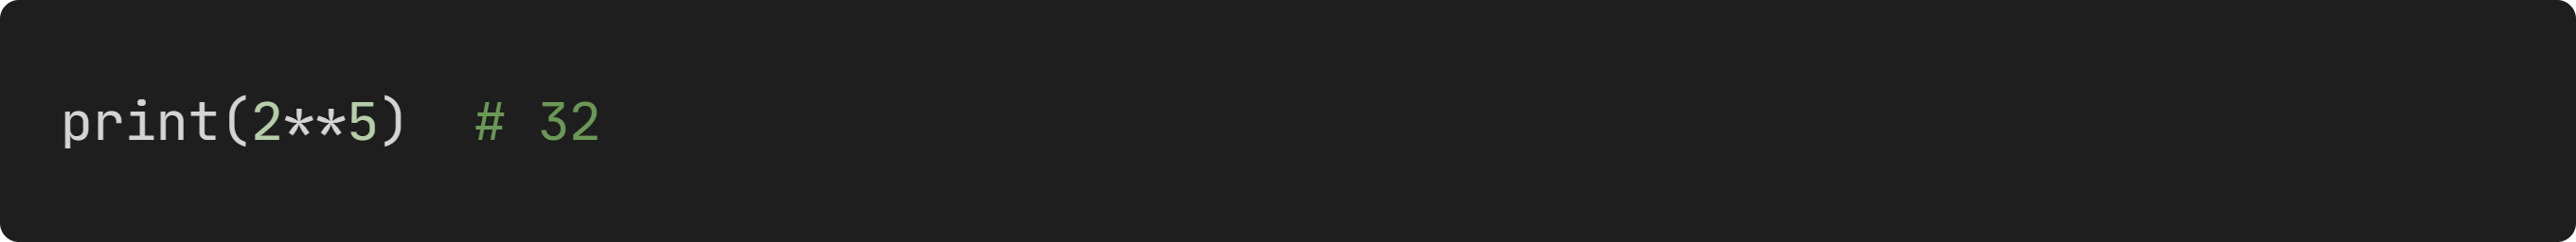
\includegraphics[width=\linewidth]{imagenes\\cap2\\potencia.png}
        \caption{Ejemplo equivalente a $2 ^ 5 = 32$.}
      \end{figure}

      \subsection{Cociente y resto}

      La división entera se realiza usando el operador //, donde el resultado es la parte entera que queda al realizar la división, también conocida como cociente.
      
      \begin{figure}[ht!]
        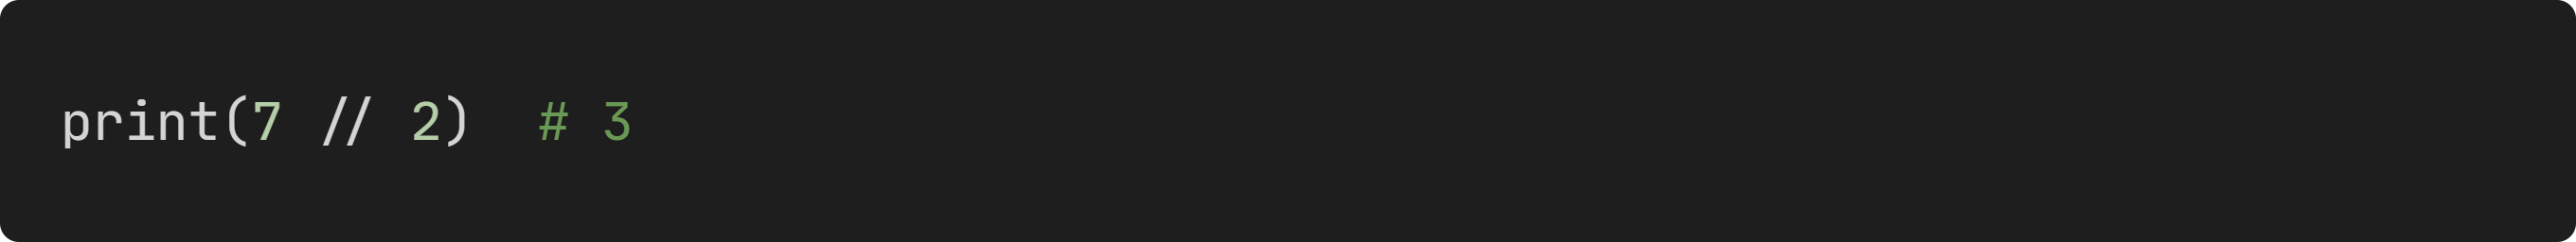
\includegraphics[width=\linewidth]{imagenes\\cap2\\cociente.png}
        \caption{La división entera retorna un entero en vez de un float.}
      \end{figure}

      Para obtener el resto al realizar una división entera, se debe usar el operador módulo \%.

      \begin{figure}[ht!]
        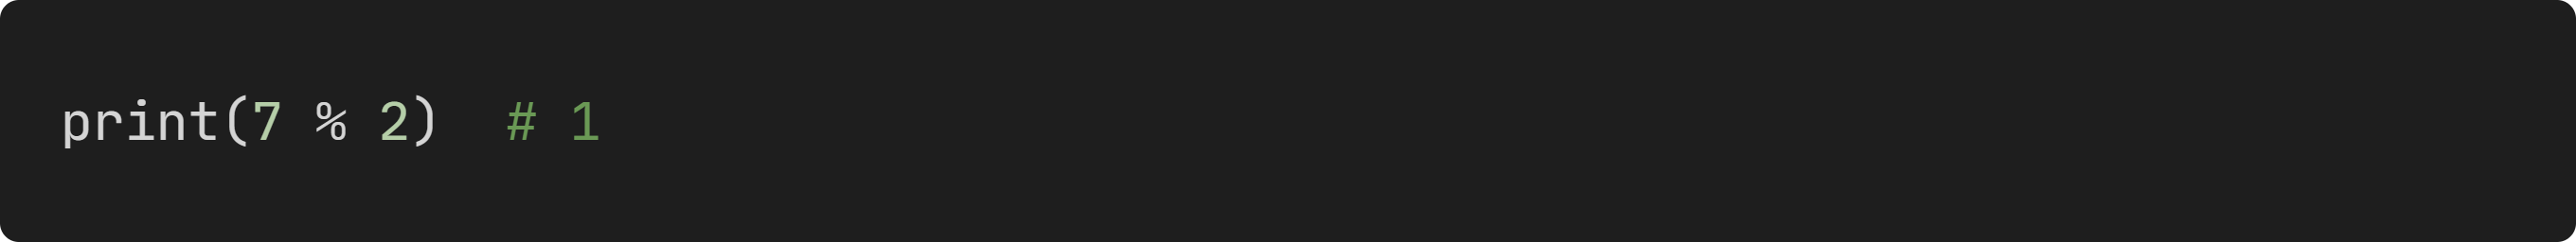
\includegraphics[width=\linewidth]{imagenes\\cap2\\resto.png}
        \caption{Esta operación es equivalente a $7 \mod{2}$ en aritmética modular.}
      \end{figure}

      Este operador viene de la aritmética modular, y uno de sus usos más comunes es para saber si un número es múltiplo de otro. Esto se hace revisando si el módulo al dividirlo por ese otro número es 0.

      \begin{figure}[ht!]
        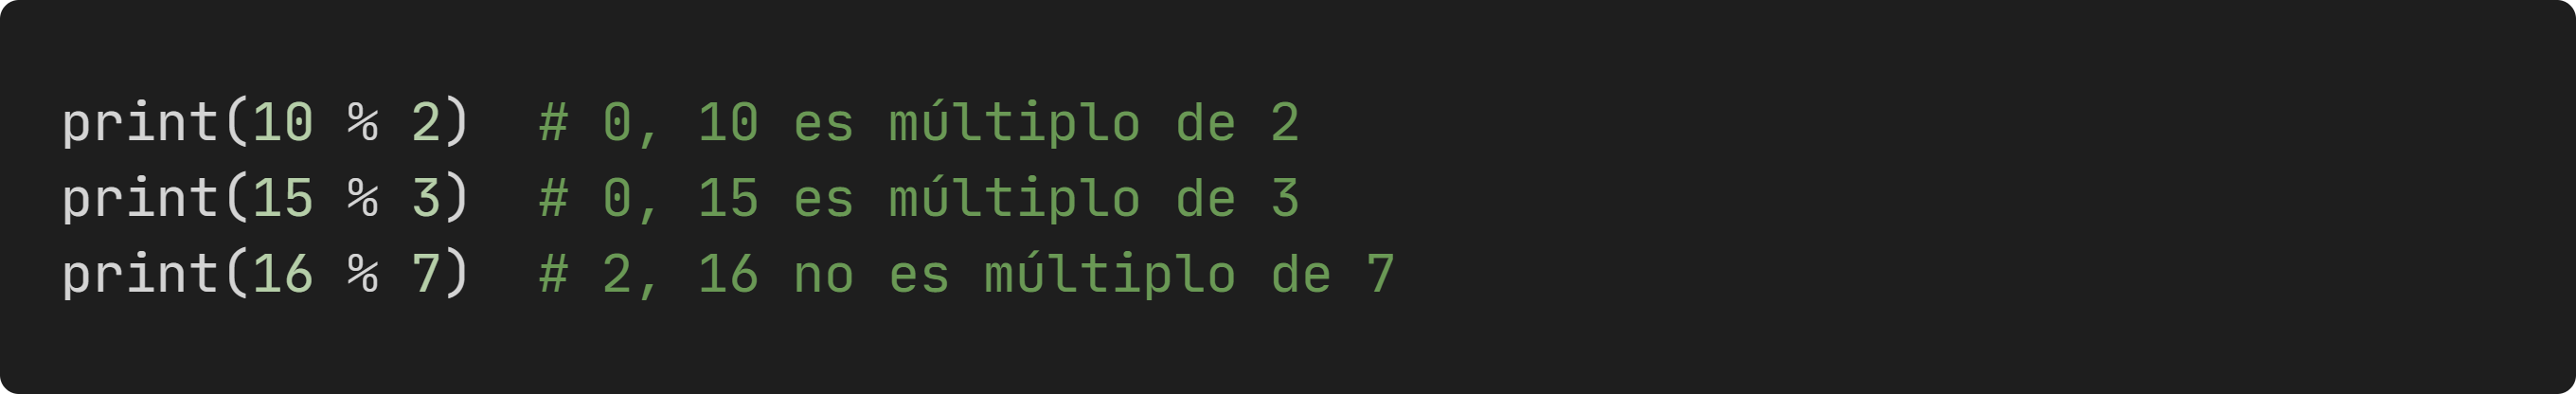
\includegraphics[width=\linewidth]{imagenes\\cap2\\uso del resto.png}
        \caption{El caso particular módulo 2 también puede usarse para saber si un número es par o no.}
      \end{figure}

    \section{Cadenas de texto}

      \subsection{Strings o cadenas de caracteres}
      \subsection{Caracteres especiales}
      \subsection{Secuencias de escape}
      \subsection{Caracteres Unicode}
      \subsection{Strings multilínea}
      \subsection{Comentarios multilínea}
      \subsection{Concatenación de strings}
      \subsection{Multiplicación de strings}
      \subsection{Opciones del método print()}
    
    \section{Variables}

      \subsection{Asignación de variables}
      \subsection{Nombre de variables válidos}
      \subsection{Palabras clave}
      \subsection{Operaciones con variables}
      \subsection{Entrada}
      \subsection{Conversión de tipos de datos}
      \subsection{Operadores de asignación}
    
    \section{Estructura de control if}

      \subsection{Booleanos}
      \subsection{Operadores de comparación}
      \subsection{Declaración if}
      \subsection{Declaración if-else}
      \subsection{Declaración elif}
      \subsection{Operadores lógicos}
      \subsection{Precedencia de operadores lógicos}

    \section{Listas}

      \subsection{Creación de listas}
      \subsection{Indexación de listas}
      \subsection{Lista vacía}
      \subsection{Anidación de listas}
      \subsection{Operaciones con listas}
      \subsection{Funciones de listas}
      \subsection{Copiar listas}
      \subsection{Strings como listas}
      \subsection{Indexación de strings}
      \subsection{Conversión de strings a listas}

    \section{Bucles}

      \subsection{Bucles while}
      \subsection{Declaración break}
      \subsection{Declaración continue}
      \subsection{Bucle for con listas}
      \subsection{Rangos}
      \subsection{Bucle for en rangos}
    
    \section{Funciones}

      \subsection{¿Qué es una función?}
      \subsection{Definición de funciones}
      \subsection{Llamado de funciones}
      \subsection{Devolución de valores en una función}
      \subsection{Docstring}
      \subsection{Funciones como objetos}
      \subsection{Sobrecarga de funciones}
      \subsection{Anotaciones de tipos}
    
    \section{Módulos y la biblioteca estándar}

      \subsection{Módulos}
      \subsection{Alias}
      \subsection{La biblioteca estándar}
      \subsection{Módulos externos y pip}
    
    \section{El módulo math}

    \section{El módulo random}

    \section{Manejo de excepciones}

      \subsection{Excepciones}
      \subsection{Declaración try-except}
      \subsection{Declaración finally}
      \subsection{Levatar excepciones}
      \subsection{Aserciones}

    \section{Pruebas unitarias}

    \section{Manejo de archivos}

      \subsection{Abrir archivos}
      \subsection{Modos de apertura}
      \subsection{Cierre de archivos}
      \subsection{Lectura de archivos}
      \subsection{Escritura de archivos}
      \subsection{Declaración with}

    \section{Módulos time y datetime}

    \section{Programación funcional}

    \section{Conjuntos y estructuras de datos}

    \section{El módulo itertools}

    \section{Programación orientada a objetos}

    \section{Expresiones regulares}

    \section{Empaquetamiento}

    \section{Interfaz gráfica}

    \section{Algoritmos de búsqueda}

    \section{Algoritmos de ordenamiento}

\end{document}